%==========================================================================

\begin{frame}[fragile]

  {\Huge Organizational}

  \vspace{15pt}

  \textbf{Content:}
  \begin{itemize}
    \item Kokkos User Group @ HPSF Conference '27 (US)
    \item Save the Date
    \item Mailing Lists
  \end{itemize}

\end{frame}

%==========================================================================

\begin{frame}[fragile]{Save The Date}

\textbf{KUG 2027 @ HPSFCon}
\begin{itemize}
\item April 12th - 16th in Montreal Canada
\item Save the date website: \url{https://events.linuxfoundation.org/hpsf-conference/}
\item Call for submissions expected mid September
\end{itemize}

\end{frame}

%==========================================================================

\begin{frame}[fragile]{Citing Kokkos - Help us track the impact of Kokkos}

\begin{itemize}
\item Ensure reproducibility
  \begin{itemize}
  \item Version-specific citations for Core and Kernels since 5.0
  \item Format: \emph{Kokkos Core v5.2.0, DOI: 10.5281/zenodo.21648054}
  \item See \href{https://kokkos.org/about/releases/}{release page} to find the specific DOI for the version you used
  \end{itemize}
\item In addition to that, please also cite relevant papers describing the component of the Ecosystem you used
\end{itemize}

Visit \url{https://kokkos.org/citing-kokkos/}

\end{frame}

%==========================================================================

\begin{frame}[fragile]{Tea-Time Webinar Series}

\begin{columns}
\column{0.5\textwidth}
\begin{itemize}
\item On the 3rd Wednesday of the month at 4 PM Paris time (usually 10 AM Eastern, 8 AM Mountain, 11 PM Tokyo time)
\item Find the playlist on \href{https://youtube.com/playlist?list=PLRKq_yxxHw2-Dkc4rEo8s-b3uaxJfuavA&si=BTBwI65FpP7B08uw}{HPSF YouTube channel}
\item Reach out if you would like to get invited to speak
\end{itemize}

\column{0.5\textwidth}
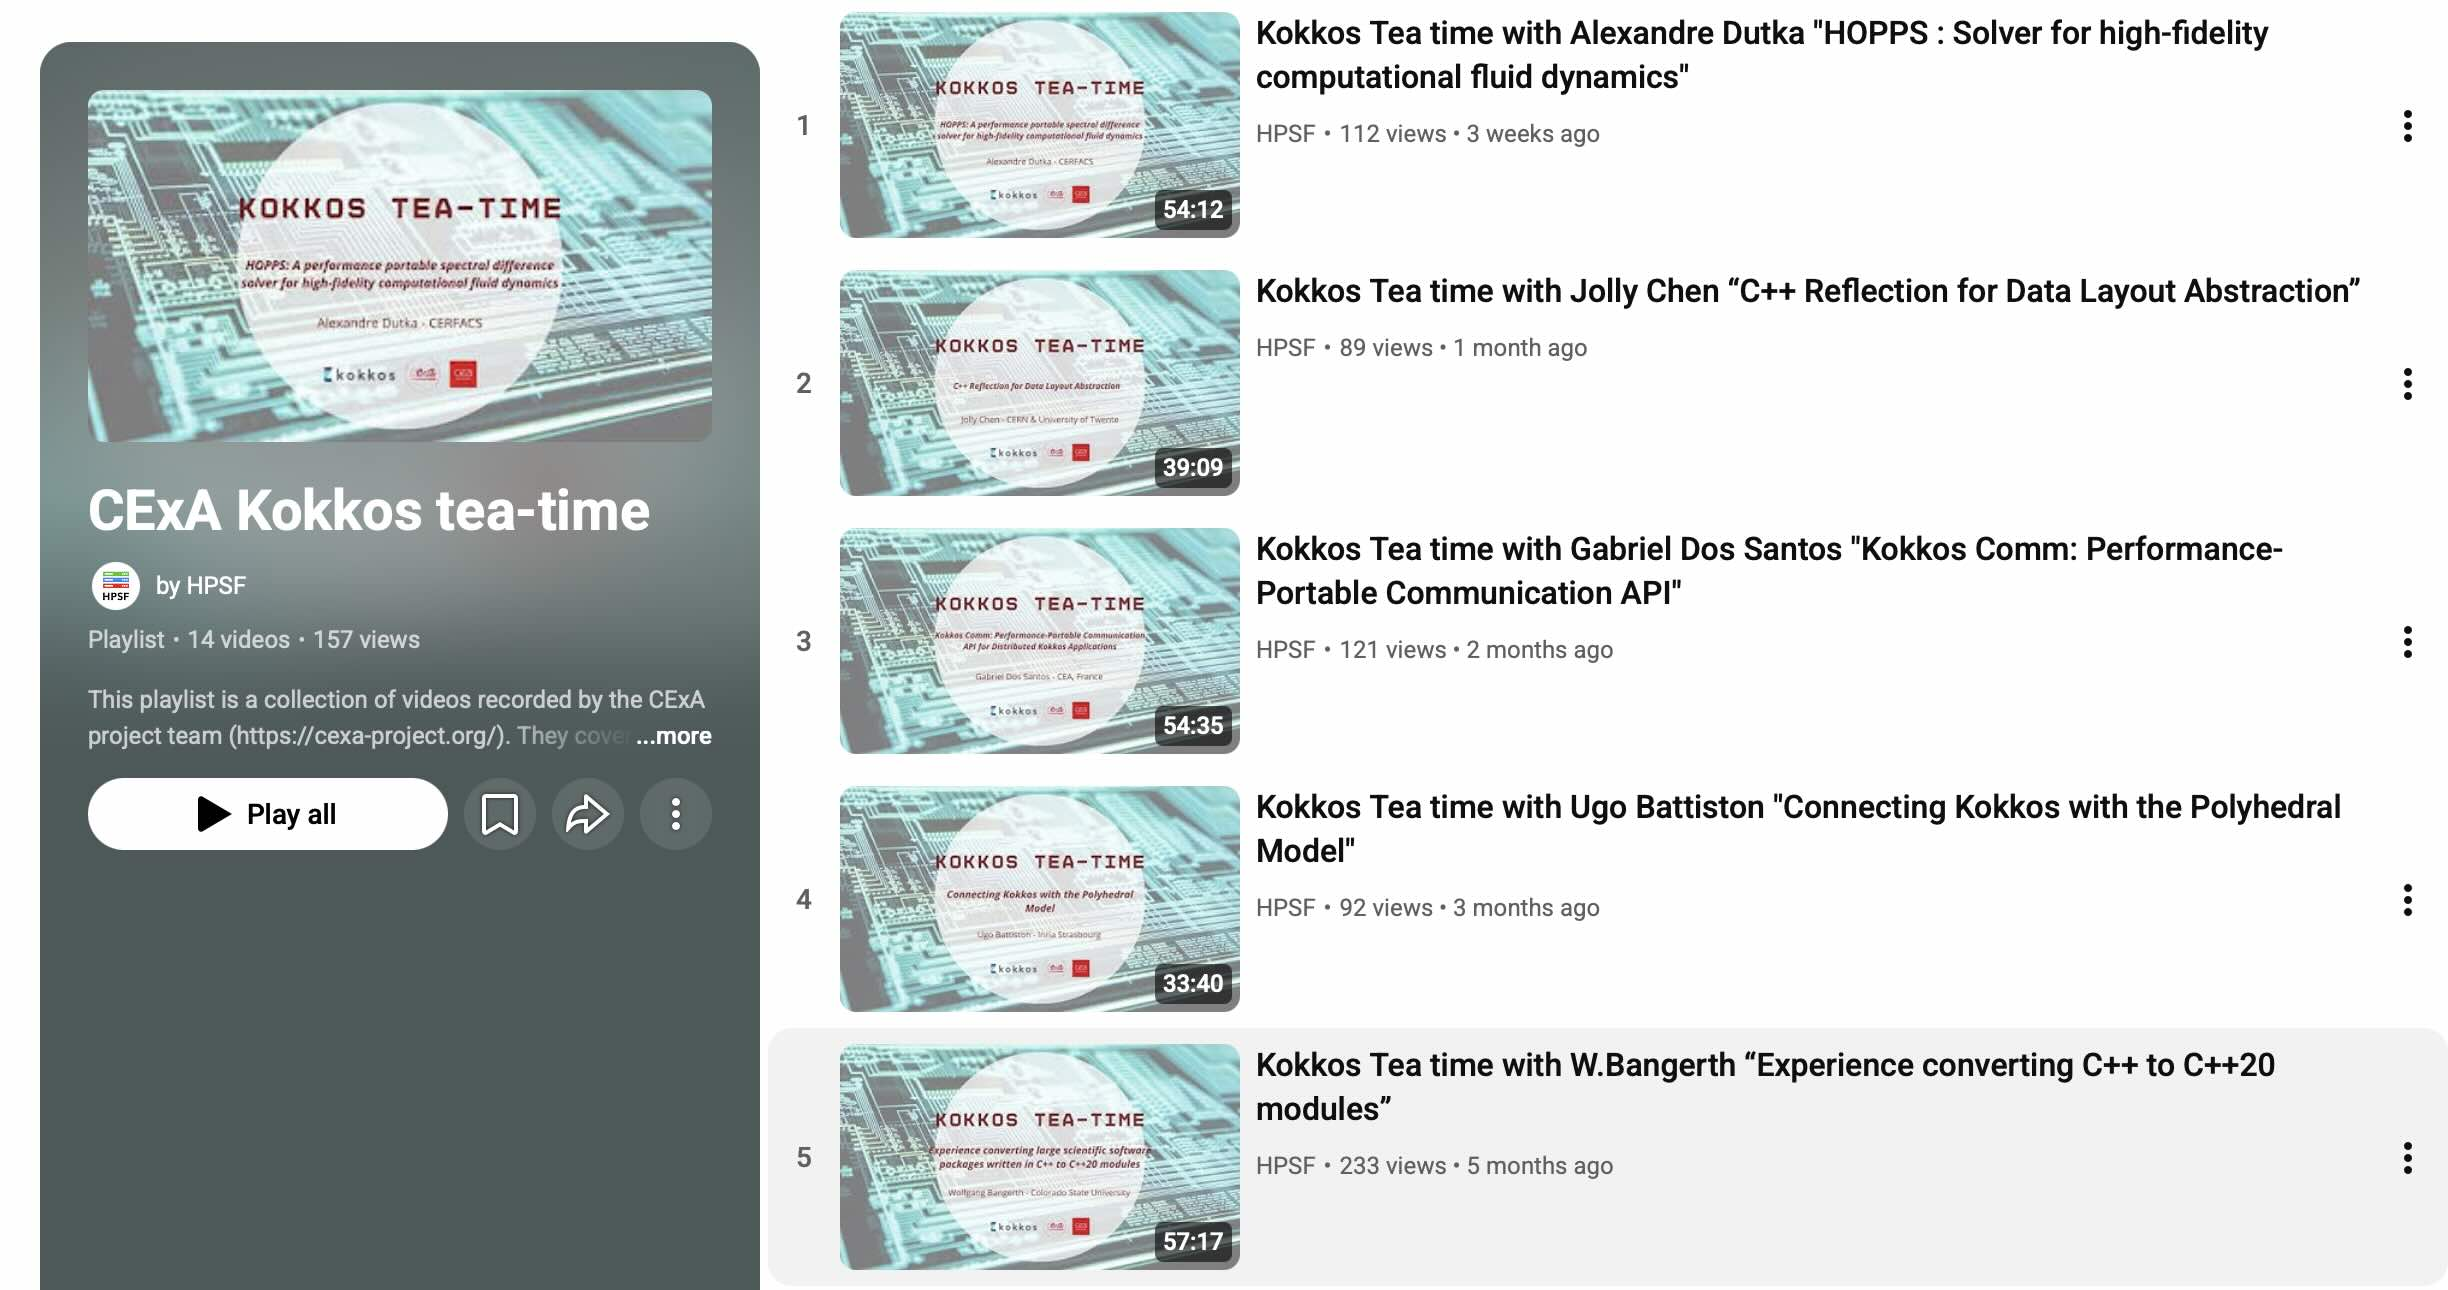
\includegraphics[width=\linewidth]{5_1/kokkos-tea-time-playlist.jpg}
\end{columns}

%\begin{block}{Next session scheduled for tomorrow}
%\emph{Parthenon – a performance portable block-structured adaptive mesh refinement framework}
%by Philipp Grete
%\end{block}

Visit \url{https://kokkos.org/community/tea-time/}

\end{frame}

%==========================================================================

% Examples

% note: always keep the [fragile] for your frames!

%\begin{frame}[fragile]{Example list}
%  \begin{itemize}
%      \item Item 1
%      \item Item 2 with some \texttt{code}
%      \begin{itemize}
%        \item Sub-item 2.1
%        \item Sub-item 2.2
%      \end{itemize}
%  \end{itemize}
%\end{frame}

%\begin{frame}[fragile]{Example code}
%    \begin{code}[keywords={std}]
%        #include <iostream>
%
%        int main() {
%            std::cout << "hello world\n";
%        }
%    \end{code}
%\end{frame}

%\begin{frame}[fragile]{Example table}
%    \begin{center}
%        \begin{tabular}{l|l}
%            a & b \\\hline
%            c & d
%        \end{tabular}
%    \end{center}
%\end{frame}

%==========================================================================

